\section{$\lgname$ case studies}

(2 pages)
\sayan{Move elsewhere. Implementation details and usage details. Mutex, controller, path planning.}
Implementation of the sensor.. GPS indoor positioning, done variable. 
%

\subsection{Platooning}
\label{sec:platooning}
In this program, the system handles automated vehicles performing platooning by communicating through shared variables. The goal of this program is to maintain at least a \emph{safe} distance between any two consecutive cars. The first car (highest pid) moves at a constant $x$ velocity. Every other car with pid $i$ sets the actuator that sets its velocity based on its distance from the car with pid $i+1$. The cars communicate through the \emph{allread} variable $\mathit{pos}$, which they update every time they execute the event \emph{SetVelocity}, or every $\delta$ time units.

\begin{figure}[ht!]
    \noindent
    \begin{center}
        \scriptsize
        \two{0.4}{0.6}
        {\lstinputlisting[language=xyzNums,firstline=1,lastline=15,frame=none]{code/platooning.tex}}
        {\lstinputlisting[language=xyzNums,firstline=16,frame=none,firstnumber=16]{code/platooning.tex}}
    \end{center}
    \caption{$\lgname$ program for robot $i$ in a Platoon to adjust its $x$ velocity accordingly .}
    \label{fig:platooningapp}
\end{figure}


\reffig{platoon} (\emph{Left}) shows $x$ vs $\mathit{time}$ plot of the program shown in \reffig{platooningapp}. In \emph{Platoon} we set the $x$ velocities based on separation, and the first car is moving at a constant velocity. As expected eventually, the cars start moving at a constant separation from each other. 
\begin{figure}[ht!]
    \noindent
    \begin{center}
        \scriptsize
        \two{0.4}{0.6}
        {\lstinputlisting[language=xyzNums,firstline=15,lastline=25,firstnumber=15,frame=none]{code/platooning2.tex}}
        {\lstinputlisting[language=xyzNums,firstline=26,frame=none,firstnumber=26,lastline=36]{code/platooning2.tex}}
    \end{center}
    \caption{ Updating the \emph{Platoon} app to include periodic velocity changes for the first car}
    \label{fig:platooningapp2}
\end{figure}

We make a small change to \emph{Platoon} to make the first car periodically switch its velocities (\reffig{platooningapp2}), and the resulting $x$ vs $\mathit{time}$ plot is shown in \reffig{platoon} (\emph{Right}).

\begin{figure}[h!]
\begin{minipage}{0.5\textwidth}
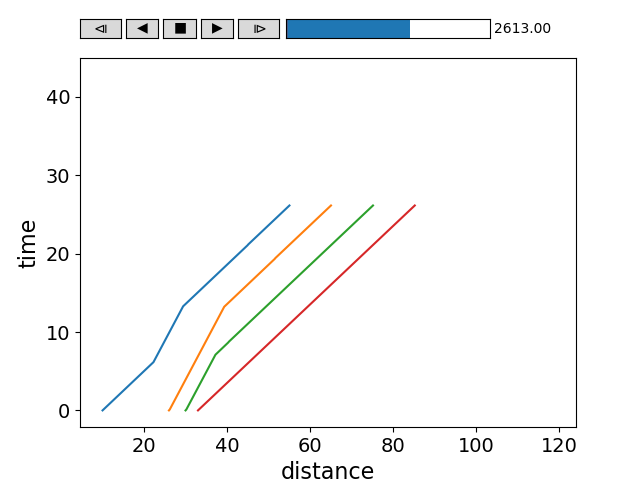
\includegraphics[width=.5\textwidth]{figs/braking_1.png}}\hfill%
%\includegraphics[width=.3\textwidth]{figs/Platooning_2.png}}\hfill%
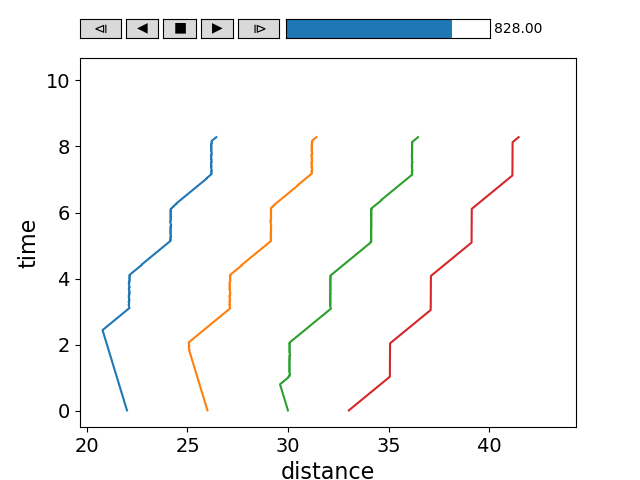
\includegraphics[width=.5\textwidth]{figs/braking_3.png}}
\end{minipage}%
	\caption{\small {Platoon of four cars. \emph{Left} shows the first car moving with a constant velocity} and \emph{Right} shows the first car switching velocities periodically.}
\label{fig:platoon}
\end{figure}

%FIGURE OUT THE VERIFICATION. 
 A \emph{correct} program should ensure that at no point, the separation along the $x$-axis between two of agents is less than the required safe distance.  Note, that the variable $\emph{safedist}$ needs to be set to higher than the actual required separation to account for reacting to the previous vehicle updating its $\mathit{pos}$ value, depending on how long the sampling parameter $\delta$ is. We  checked that \emph{Platoon}(\reffig{platooningapp}) was indeed safe for frequent sampling, i.e, when $\delta$ is small enough and the variable $\emph{pos}$ is updated frequently, and unsafe otherwise.  \reffig{unsafeplatoon} shows the $x$ vs $\mathit{time}$ when the cars react too slowly.

\begin{figure}[h!]
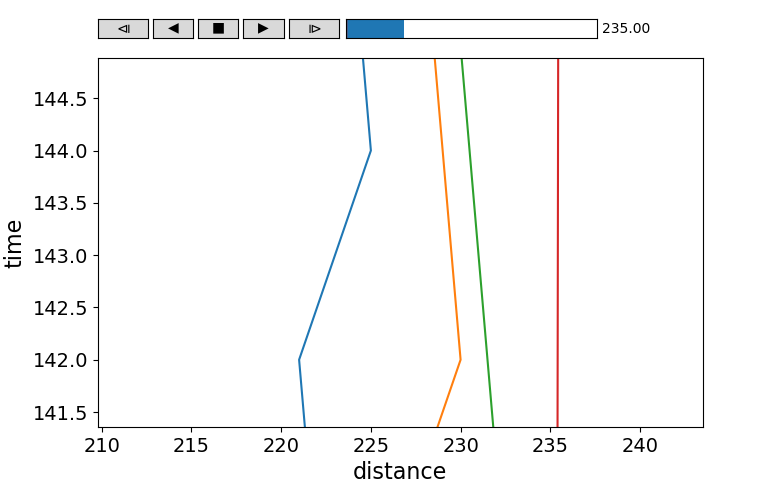
\includegraphics[scale=0.3]{figs/unsafe_braking.png}
	\caption{\small {Platoon of four cars. \emph{Left} shows the first car moving with a constant velocity} and \emph{Right} shows the first car switching velocities periodically.}
\label{fig:unsafeplatoon}
\end{figure}

\subsection{Formation: portability}
\label{sec:formation}

Simplicity of code because of shared variables.

Logs, visualized.

\subsection{Task: portability and heterogeneous}

Figures screenshots. 

Numbers, Change motion model and sensor? 


Convergence time, task completion time.



Mutual exclusion is always an essential feature when shared variables are involved. $\lgname$ provides a locking mechanism using the keyword $\mathit{atomic}$, which the $\mathit{Assign}$ event uses to update the shared list of tasks $\mathit{taskList}$ safely. $\lgname$ supports two types of shared variables, multiwriter-multireader (\emph{allwrite}), and singlewriter-multireader (\emph{allread}) shared variables, whose functionality is as their names suggest. 
 %
The implementation of $\mathit{Motion}$ controller involves, for example, path planners, and platform-specific steering and throttle controllers, and drivers for specific positioning systems. 

We developed a simulator \reffig{simulator} for $\lgname$ applications within the CyPhyHouse framework to enable the user a way of testing their discrete event loop with simple motion models to test and debug the application program logic. The CyPhyHouse simulator uses motion automata, which can be provided any programmable dynamics to simulate the robot dynamics. The simulated sensed data is also provided realistic noises and dynamics to mimic actual system dynamics. The communication protocols are also a part of the simulator communication module. The time between two computational steps (or discrete event loop iterations) is used to propagate messages to implement shared memory as in the actual hardware stack.
\subsection{benchmarks}
\subsection{variations}
\subsection{results}